

\documentclass{article}
\renewcommand*\familydefault{\ttdefault}
\usepackage[T1]{fontenc}
\usepackage[right=1cm, left=1cm, top=1cm, bottom=2cm]{geometry}
\usepackage{parskip}
\usepackage{circuitikz}

\usepackage{listings}
\usepackage{mathtools}
\usepackage{relsize}
\usepackage{graphicx}
\usepackage{float}
\usepackage{pgfplots}\pgfplotsset{compat = 1.18}

\title{Software Enginnering Fall 2023-2024 \\ Valuni Requirements Specification}
\author{  
Hussein Heggi 	\and
Ahmed Waseem Raslan 	\and
Sarah Elsamanody 	\and
Nour Abdalla 	\and
Youssef Elmahdy	\and
Ahmed Elbarbary	\and 
Ahmed Jaheen}


\begin{document}

\maketitle 

\break

\section*{Project Description}
VALUNI is a platform where students have the opportunity to share their experiences and exchange knowledge and feedback regarding both professors and courses.  It would play a vital role in helping students hold sufficient knowledge that could ease up the process of choosing classes and preparing for exams. Our objective is to create a safe, dependable and organized environment that allows students to express their opinions in an honest and respectful way. We aim to motivate students when rating or writing their reviews through anonymity, and at the same time having certain guidelines that must be followed when using VALUNI. This will not only assist students, but also the overall University community including diverse facilities and professors. 

\section{Product Backlog}

\subsection{Functional Requirements}

	\quad User authentication 
	\vspace{-0.2cm}

	\qquad \scriptsize User login and verification that user is a university student \normalsize

	\quad Rating Courses

	\quad Rating Professors

	\quad Writing out a review with Rating
	\vspace{-0.2cm}

	\qquad \scriptsize When Reviewing students have the option to write a review with the parameterized rating \normalsize

	\quad Parameterized Rating
	\vspace{-0.2cm}

	\qquad \scriptsize Students can rate professors and courses on different parameters, such as workload, leniency \normalsize

	\quad Filtered Search on parameters 
	\vspace{-0.2cm}

	\qquad \scriptsize Students can filter out result or search for courses and professors based on parameters \normalsize

	\quad Reporting reviews

	\quad Editing Reviews

	\quad Admin ( university ) access to review data 
	\vspace{-0.2cm} 

	\qquad \scriptsize University can access critical semster review analytics as well as overall analytics \normalsize

	\quad Search for courses 

	\quad Search for professors 



\subsection{Non Functional Requirements} 

	\quad Fluid, Simple UI

	\quad Secure

	\quad Auto removing profanity on reviews

	\quad Prevent Review Bombing

	\quad Anonymous

	\quad Customer Service ( for universities )

	\quad Performance

	\quad Scalability

\section{Use Case Diagram} 

\begin{center}
	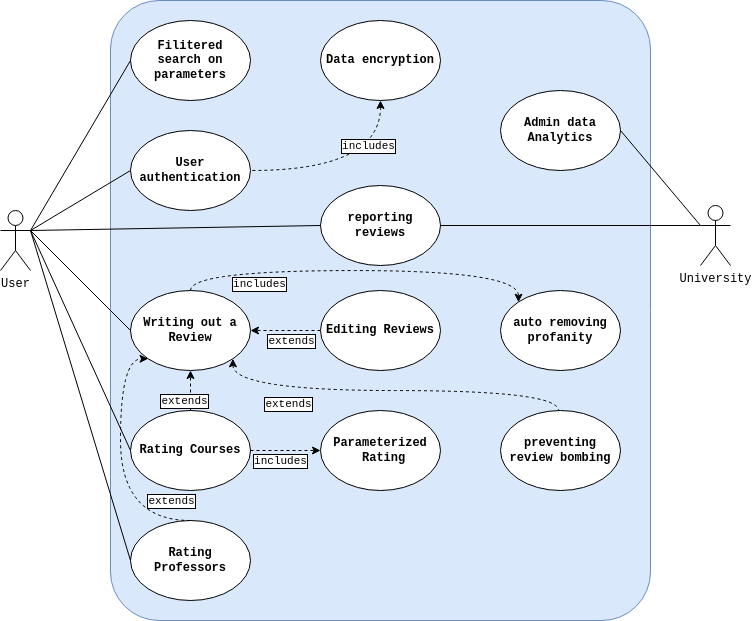
\includegraphics[scale=0.5]{./USECASE.drawio.png}	
\end{center}

\section{MVP Requirements}

	\quad User authentication (login etc)

	\quad User data encryption

	\quad Rating Courses

	\quad Rating Professors

	\quad Writing out a review with Rating

	\quad Parameterized Rating

	\quad Filtered Search on parameters	

	\quad Editing Reviews




\section{Conclusion}






\end{document}

